\chapter{\label{ch:dev}Development practices}

As this is a new software project, we invested a significant effort in setting
up a development infrastructure to ensure our work is carefully tracked,
thoroughly and continually tested, and incrementally improved and documented.
To this end, we have adopted best practices for software development used by
successful open source projects \cite{millman2014}.

\section{\label{sec:vc}Version control}

We are using Git\footnote{\url{http://git-scm.com}} as our version control
system and GitHub\footnote{\url{https://github.com}} as the public hosting
service for our official \texttt{upstream} repository.  Git allows us to
carefully track how our code evolves as well as deliberately consider 

\subsection{Workflow}

Rather than work on the \texttt{master} branch of our repositories,
we have adopted the policy of performing all code changes on
feature branches.

\subsection{Pull requests}

To get new code integrated in the official \texttt{upstream} master, we use
GitHub's \emph{pull request} mechanism.  This helps make performing code review
for new code added to the official ``upstream'' repository easy to manage.
Given the short development history and small development team, we have 

\section{\label{sec:test}Testing}

We use the \texttt{nose} testing framework for automating our testing
procedures.\footnote{\url{https://nose.readthedocs.org}}  This is the standard
testing framework used by the core packages in the scientific Python ecosystem.

For example, from the top-level of the repository, you can ask \texttt{nose}
to run the tests by entering \texttt{nosetests permute} in Bash.  For example,

\begin{verbatim}
$ nosetests permute
.......................................
----------------------------------------------------------------------
Ran 39 tests in 48.957s
\end{verbatim}

In the above console output, you will see a ``.'' for each test, which
is run.  A test corresponds to a function and each test may test several
things.

\subsection{Coverage}

We also use \texttt{nose} to monitor our test coverage.  Our goal is to
test every line of code.  For example, not only do we want to test every
function in our package, but if a specific function has internal logic
we want to test each possible path through the function.  Having tested
each line of code increases our confidence in our codebase, but more
importantly provides us assurance that changes we make do not break
existing code.  It also increases our confidence the new code works,
which reduces the friction of accepting contributions.

Working in the top-level of our local repository in Bash, you could
enter

\begin{verbatim}
$ nosetests permute --with-coverage --cover-package=permute
.......................................
Name                 Stmts   Miss Branch BrMiss  Cover   Missing
----------------------------------------------------------------
permute                 43      5     10      1    89%   77-88
permute.core            60      0     30      4    96%   
permute.data            45      0      2      0   100%   
permute.eda             22      0      8      0   100%   
permute.irr             52      0     20      1    99%   
permute.stratified      45      0     16      1    98%   
permute.utils           10      0      6      0   100%   
----------------------------------------------------------------
TOTAL                  277      5     92      7    97%   
----------------------------------------------------------------------
Ran 39 tests in 56.023s

OK
\end{verbatim}
Here you can see, that in addition to running 39 tests without error,
that over 97\% of our code has at least one test touch it.  The remaining
lines are mostly branch misses where the branch is difficult to achieve.
For example, the branch depends on the particular circumstance in which
it is being run. So each branch is tested in different circumstances, but
not at the same time. I've tried to trick the tests to run both branches by
hand modifying system objects in the tests as well as creating mock objects,
but haven't been able to achieve 100\% coverage.

\subsection{Continuous integration}

Travis CI\footnote{\url{https://travis-ci.org}}


\texttt{coveralls}\footnote{\url{https://coveralls.io}}

\begin{figure}
  \begin{centering}
    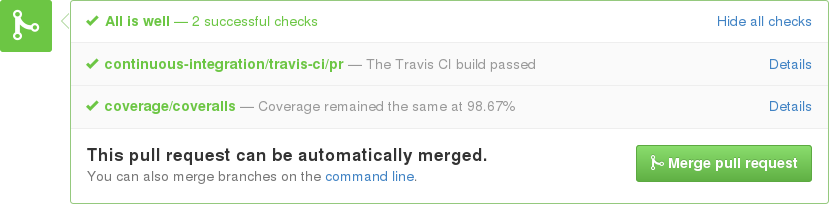
\includegraphics[width=5.5in]{fig/pull-request-ci.png}\par
  \end{centering}

  \caption{\label{fig:pull-request}Pull request and continuous integration.}
\end{figure}

\section{\label{sec:doc}Documentation}

Docstring standard \cite{SciPyProceedings_27}.

ReStructured Text

\texttt{sphinx}

\section{\label{sec:release}Release management}

